%% Computers in Human Behavior — elsarticle with APA (author-year) citations
%% Double-anonymized: this is the ANONYMIZED manuscript file
%% Submit title page with author info separately
\documentclass[review,12pt,authoryear]{elsarticle}

\usepackage{lineno,hyperref}
\usepackage{booktabs}
\usepackage{amsmath}
\usepackage{graphicx}
\usepackage{multirow}
\modulolinenumbers[5]

\journal{Computers in Human Behavior}

%% APA-style bibliography
\bibliographystyle{elsarticle-harv}

\begin{document}

\begin{frontmatter}

\title{Surfacing Suicidal Vulnerability Through Simulated Social Interaction: Per-Person Language Model Agents as Communicative Stress Tests}

%% Authors removed for double-anonymized review

\begin{abstract}
Suicidal vulnerability may be encoded in everyday communication patterns but diluted in routine digital interactions. We introduce a method for surfacing this latent signal: training per-person language model agents on individuals' real text messages and placing them in simulated social interactions---a ``communicative stress test.'' Using data from 79 adults with recent suicidal ideation, we fine-tuned individual low-rank adaptation (LoRA) adapters on an open-source language model (Qwen3-8B), then evaluated three paradigms: an all-pairs arena (2,485 paired conversations across 71 agents), a caption-trained comparison (agents trained on VLM-generated screenshot descriptions rather than messages), and a standardized probe arena (5 theory-driven personas $\times$ 71 agents). Message-trained agents whose real-world counterparts had higher ecological momentary assessment (EMA)-measured suicidal ideation produced significantly more suicide-relevant language (Spearman $\rho = .438$, $p < .001$; Cohen's $d = 0.77$), with absolutist language as the strongest single predictor ($r = .607$, $p < .001$). The standardized probe arena predicted suicidal ideation at $r = .576$ ($p < .001$), compared to $r = .477$ for the all-pairs arena and $r = .461$ for raw messages. Strikingly, a single neutral small-talk probe---with no emotional provocation---performed nearly as well ($r = .551$), and combining just two probes (Neutral Acquaintance and Supportive Therapist) yielded the best cross-validated prediction (LOOCV $r = .570$), with additional probes adding noise rather than signal. Theory-driven construct-specific probe targeting largely failed: probes designed to elicit specific interpersonal constructs did not outperform the unstructured arena for their target outcomes. Caption-trained agents produced no clinical signal despite 50$\times$ more training data, confirming that the predictive validity is specifically attributable to interpersonal communication patterns. Validation analyses confirmed that the clinical signal is person-specific: shuffling adapters across participants eliminated prediction ($r = .071$, $p = .577$), while the mismatched adapter's output tracked the adapter-owner's SI ($r = .426$, $p < .001$). A prompt ablation demonstrated that the signal partially survives without disclosure-encouraging language ($r = .430$ vs.\ $r = .576$), indicating that the prompt amplifies an existing signal rather than creating it. A no-LoRA floor control established that the base model produces near-zero between-person variance in risk language; the adapter's contribution is individual differentiation, not mean-level risk. The method systematically excludes the highest-risk participants who text least (excluded SI $M = 8.80$ vs.\ included $M = 1.80$), a fundamental limitation of text-based approaches. Temporal split validation demonstrated moderate stability (Spearman-Brown $= .538$), with both halves independently predicting SI. These findings demonstrate that simulated social interaction can amplify latent vulnerability signals in a proof-of-concept that bridges digital phenotyping, generative AI, and suicide theory.
\end{abstract}

\begin{keyword}
suicidal ideation \sep large language models \sep generative agents \sep digital phenotyping \sep interpersonal theory of suicide \sep ecological momentary assessment
\end{keyword}

\end{frontmatter}

\linenumbers

\section{Introduction}

Suicide remains a leading cause of death globally, and predicting who is at risk continues to be one of the most difficult problems in clinical science \citep{franklin2017risk}. Despite decades of research, clinicians perform only marginally better than chance at predicting suicidal behavior \citep{large2017meta}, and traditional risk factor approaches have reached apparent ceiling effects in predictive accuracy \citep{belsher2019prediction}. A central challenge is that suicidal ideation fluctuates rapidly---on the order of hours \citep{kleiman2017examination}---and the interpersonal processes theorized to drive it (perceived burdensomeness, thwarted belonging; \citealt{joiner2005why}; \citealt{vanorden2010interpersonal}) are inherently relational, manifesting most clearly in social interaction rather than in static self-report.

Two converging developments create new opportunities for studying these dynamics. First, the emergence of large language models (LLMs) capable of producing human-like text has enabled a new class of research: generative agent simulation. \citet{park2023generative} demonstrated that LLM-powered agents placed in a shared environment exhibit emergent social behaviors---organizing events, forming opinions, spreading information---without explicit programming. Subsequent work has scaled this to 1,000 agents parameterized from real interview data, achieving 85\% behavioral fidelity \citep{park2024generative}. Applications to mental health have begun to appear, including agent-based simulations of student wellbeing initialized from smartphone sensing data \citep{zhao2025studentlife} and conceptual frameworks for modeling socio-environmental determinants of mental health \citep{kambeitz2025modelling}. Concurrently, there has been a rapid expansion of LLMs applied directly to suicide prevention \citep{holmes2025scoping}.

A growing body of work has explored using LLMs as proxies for human participants more broadly. \citet{argyle2023silicon} introduced ``silicon sampling,'' conditioning LLMs on demographic descriptions to simulate survey responses and coining the term ``algorithmic fidelity.'' \citet{aher2023turing} proposed ``Turing Experiments,'' evaluating LLMs as stand-ins for human subjects in classic psychology paradigms, finding both promising alignment and a systematic ``hyper-accuracy distortion.'' In psychological assessment, \citet{peters2024llm} demonstrated that GPT-3.5 and GPT-4 can infer Big Five traits from Facebook posts ($r = 0.29$), and \citet{brickman2025llm} provided a comprehensive review introducing the concept of ``LLM rating scales.''

Applications to mental health simulation have begun to appear but remain limited. \citet{qiu2025emoagent} developed EmoAgent, simulating vulnerable users interacting with AI chatbots and finding that over 34\% showed psychological deterioration---the closest analog to our ``stress test'' concept, though EmoAgent tests the safety of AI chatbots rather than creating personalized agents from individual behavioral data. \citet{louie2024roleplay} took a complementary approach with Roleplay-doh, in which domain experts crafted principles for LLM-simulated patients, validating the use of carefully designed probe personas. However, \citet{tornberg2025validation} offered a critical review arguing that LLMs may exacerbate rather than solve the validation challenges inherent in agent-based social simulation.

A key distinction separates this prior work from our approach. Existing agent simulation methods rely on \textit{prompt-based conditioning}---providing demographic descriptions \citep{argyle2023silicon}, interview transcripts \citep{park2024generative}, or expert-designed persona specifications \citep{louie2024roleplay}---to shape model behavior. This approach faces a fundamental individuation problem. \citet{peng2025funhouse} characterized digital twins created through prompting as ``funhouse mirrors,'' identifying five systematic distortions and finding that the average correlation between digital twin and real human responses is only $r = 0.20$. \citet{li2025behaviorchain} developed BehaviorChain, the first benchmark for persona-based behavior simulation, demonstrating that even state-of-the-art models struggle to maintain behavioral consistency across extended interaction chains. Our approach differs fundamentally: rather than conditioning a model through prompts, we \textit{fine-tune} per-person LoRA adapters on each individual's actual text messages, learning directly from behavioral data rather than from descriptions of behavior. This may overcome the ``insufficient individuation'' that prompting-based approaches suffer from, precisely because the adaptation occurs at the level of model weights rather than context.

Second, digital phenotyping---the continuous measurement of behavior through smartphones and wearable sensors---has produced rich longitudinal records of how individuals communicate in daily life. Screenomics, which captures smartphone screenshots at five-second intervals \citep{reeves2021screenomics}, provides near-complete records of text messages sent and received. When combined with ecological momentary assessment (EMA) of suicidal ideation, these data reveal moment-to-moment relationships between digital communication and suicide risk \citep{ammerman2026beyond}. However, analyzing raw message content for suicide risk faces fundamental limitations: most messages are logistical and routine, risk-relevant content is sparse and diluted, and direct surveillance of private messages raises profound ethical concerns.

We propose a novel approach that bridges these two developments: training per-person language model agents on individuals' actual text messages and then placing those agents in simulated social interactions to surface latent communication patterns associated with suicidal vulnerability (Figure~\ref{fig:paradigm}). The key insight is that a language model fine-tuned on someone's messages learns not just the content of any specific conversation but the probability distribution over how that person communicates---their word choices, emotional expression patterns, relational tendencies, and cognitive style. We conceptualize this as a \textit{communicative stress test}---analogous to cardiac stress testing, where a resting ECG may appear normal but underlying vulnerability becomes visible under exertion. In our paradigm, routine text messages are the resting state, and the simulated conversation is the treadmill.

\begin{figure*}[t]
    \centering
    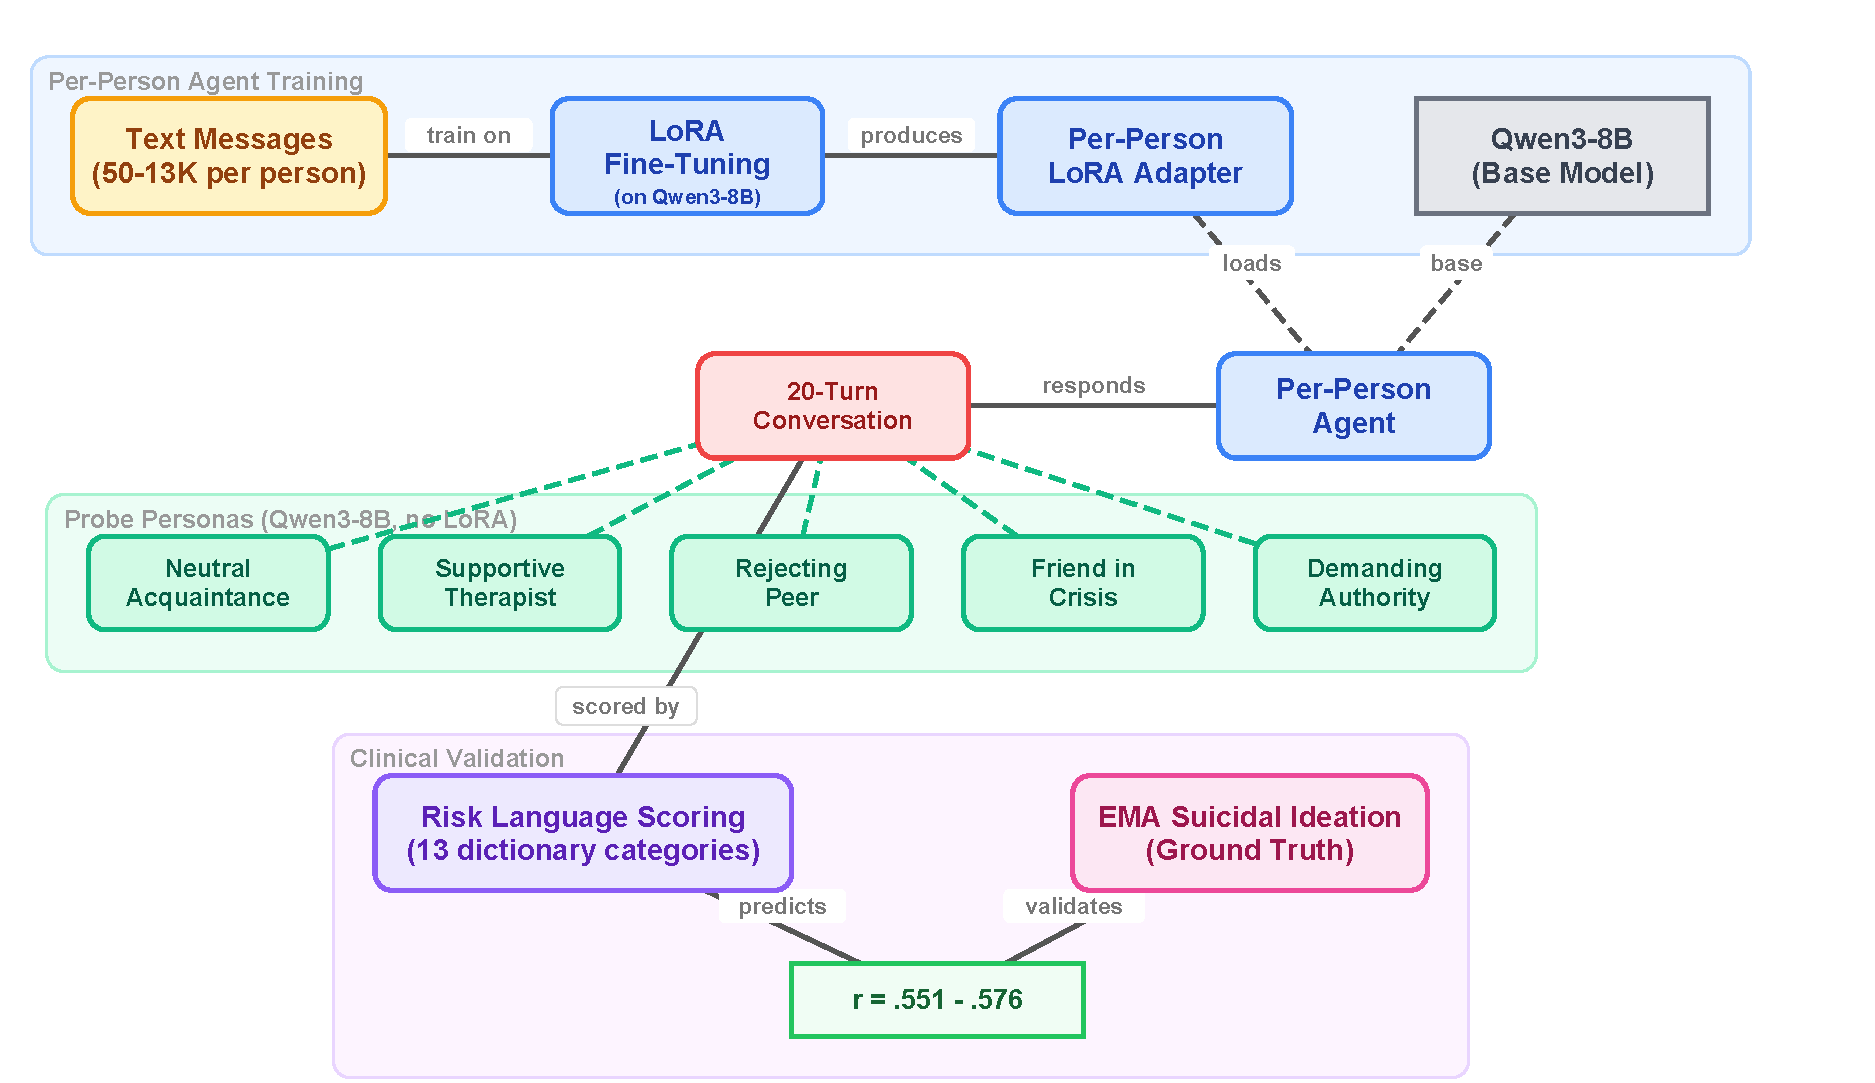
\includegraphics[width=0.95\textwidth]{figures/fig1_paradigm_overview.pdf}
    \caption{Overview of the communicative stress test paradigm. Per-person LoRA adapters are trained on each participant's real text messages, then loaded onto a base language model to create individualized agents. Each agent engages in 20-turn conversations with standardized probe personas. The generated text is scored with risk language dictionaries and correlated with EMA-measured suicidal ideation.}
    \label{fig:paradigm}
\end{figure*}

This approach is grounded in two theoretical foundations. First, the Interpersonal Theory of Suicide (ITS; \citealt{joiner2005why}; \citealt{vanorden2010interpersonal}) posits that the desire for suicide arises from the simultaneous presence of perceived burdensomeness and thwarted belonging---both inherently interpersonal constructs. If these constructs are reflected in communication patterns, they should manifest more clearly in social interaction than in static text analysis. Second, a substantial psycholinguistic literature has established that language carries reliable markers of suicidal risk. Seminal work by \citet{stirman2001word} demonstrated that suicidal poets used more first-person singular pronouns and fewer first-person plural pronouns than non-suicidal poets. \citet{almosaiwi2018absolute} showed that absolutist thinking---operationalized through words like ``nothing,'' ``completely,'' and ``always''---is a cognitive-linguistic marker specific to suicidal ideation beyond what negative emotion words alone capture. More broadly, a systematic review \citep{ophir2022linguistic} identified consistent markers across studies, including elevated self-referential language, death-related vocabulary, and reduced future-oriented words.

Dictionary-based approaches have been central to translating these findings into applied risk detection. The Linguistic Inquiry and Word Count (LIWC; \citealt{pennebaker2015development}) program remains the most widely used tool, with validated applications to suicide notes \citep{pestian2012sentiment}, crisis hotline transcripts \citep{huang2024mindsets}, and clinical interviews \citep{tausczik2010psychological}. In clinical messaging contexts, \citet{swaminathan2023nlp} demonstrated that a two-stage NLP system combining keyword filtering with machine learning reduced crisis message triage time from 9 hours to 8--13 minutes. In our own prior work, we applied dictionary-based classification to text messages extracted from smartphone screenshots, finding that within-person increases in negative emotional expressions co-occurred with elevated suicidal ideation \citep{ammerman2026beyond}. The present study extends this dictionary-based approach from classifying existing messages to scoring language \textit{generated} by per-person LLM agents.

The present study addresses six primary questions. First, do per-person fine-tuned language model agents produce risk-relevant language at rates that predict their real-world counterparts' suicidal ideation? Second, does the arena provide incremental predictive validity over direct analysis of participants' actual text messages? Third, is the predictive signal specific to interpersonal communication style, or would any behavioral data suffice? Fourth, do standardized conversational probes---designed to target specific ITS constructs---differentiate from the unstructured all-pairs arena, and does construct-specific scoring improve prediction? Fifth, are the adapters person-specific, such that clinical prediction depends on correct person--adapter matching? Sixth, does the learned communication style reflect stable individual differences or transient states?


\section{Method}

\subsection{Participants and Procedure}

Participants were 79 adults (ages 18--65) recruited from the community who endorsed past-month active suicidal ideation or suicidal behaviors and owned an Android-based smartphone. Full eligibility criteria and recruitment procedures are described in [blinded for review]. Following a baseline assessment, participants completed 6 EMA prompts per day for 28 days (overall response rate = 68.8\%). Simultaneously, a passive sensing application captured screenshots at five-second intervals during active smartphone use, yielding approximately 7.4 million screenshots across the sample ($M = 92{,}613$ per participant).

\subsection{Message Extraction}

Text messages were extracted from screenshots using a vision-language model (VLM) pipeline. Specifically, the Qwen2.5-VL-7B-Instruct model \citep{qwen2025qwen3} processed each screenshot with a structured prompt that (a) detected the presence of a keyboard, indicating an active messaging context, and (b) when a keyboard was detected, extracted message text separately for the phone owner (typically displayed in right-aligned dialogue boxes) and the message recipient (typically left-aligned). Validation against 500 human-annotated screenshots demonstrated 99.7\% accuracy for keyboard detection, and when keyboards were present, 100\% accuracy for text extraction from both owner and recipient messages. This pipeline produced two text streams per participant---\textit{owner text} (messages sent by the participant) and \textit{recipient text} (messages received).

\subsection{EMA Measures}

At each EMA prompt, participants reported on suicidal ideation using four items assessing passive ideation (wishes for death, thoughts of death) and active ideation (thoughts of killing oneself, intent to act). Additional items assessed suicidal planning (3 items), desire for death (2 items), perceived burdensomeness (2 items), thwarted belonging (2 items), positive affect (10 items from the PANAS), and negative affect (12 items). All items were summed within construct at each prompt, then aggregated to person-level means and standard deviations.

\subsection{Per-Person Agent Training}

\subsubsection{Message Filtering}

For each participant, sent (owner) text messages were cleaned in two stages. First, messages shorter than five characters, empty strings, and VLM output artifacts were removed. Artifact filtering targeted 16 patterns characteristic of VLM extraction failures. Second, a minimum message count threshold of 50 post-filtering messages was applied. Of the 79 participants, 73 met this threshold. Among eligible participants, message counts varied substantially ($Mdn = 733$; $M = 1{,}983$; range = 50--13,551). LoRA training was attempted for all 73; two failed to converge, yielding 71 agents with successful adapters. Of these, 64 could be matched with valid EMA data.

\subsubsection{LoRA Fine-Tuning}

We used Qwen3-8B \citep{qwen2025qwen3} as the base language model. For each participant, we trained a low-rank adaptation (LoRA; \citealt{hu2022lora}) adapter on that individual's cleaned owner messages. LoRA modifies a small number of parameters (rank $r = 8$, $\alpha = 16$, targeting the query and value projection matrices) while keeping the base model frozen. Each adapter was trained for 3 epochs with a causal language modeling objective. No clinical labels were provided during training; the model learned only from raw message text.

\subsection{Arena Paradigms}

We evaluated three conversational paradigms of increasing structure, each using the same per-person LoRA adapters and identical generation parameters (temperature $= 0.9$, top-$p = 0.95$, repetition penalty $= 1.3$, maximum 200 new tokens per turn). All conversations were scored using the same two-layer dictionary system described below.

\subsubsection{Paradigm 1: All-Pairs Arena}

Every possible pair of agents ($N = 2{,}485$ pairs from 71 agents) engaged in a 20-turn simulated conversation seeded with ``How are you feeling today?'' Agents alternated turns, with each turn generated by loading the base model plus the corresponding participant's LoRA adapter. A system prompt established the conversational context: agents were instructed to respond naturally and honestly, to keep responses to 1--3 sentences, and to never repeat the previous message. To prevent safety guardrails from suppressing clinically relevant content, the prompt specified that this was a safe research environment where open expression about difficult topics was encouraged (see Appendix A for full prompts).

\subsubsection{Paradigm 2: Caption-Trained Arena}

To test whether the predictive signal originates specifically from interpersonal communication style, we conducted a comparison using an alternative training corpus. For each participant, the Qwen2.5-VL-7B-Instruct VLM had previously generated natural-language descriptions of every screenshot (approximately 93K per participant), characterizing application usage, content viewed, messaging context, and temporal patterns. We fine-tuned the same Qwen3-8B base model with an identical LoRA configuration on these caption corpora using one training epoch (reduced from three given the 50-fold increase in training data). Sixty-seven participants yielded successful caption-trained adapters. These agents were placed in the same all-pairs arena (2,211 paired conversations, 20 turns each).

\subsubsection{Paradigm 3: Standardized Probe Arena}

To test whether structured conversational probes designed to elicit specific ITS constructs could outperform the unstructured all-pairs arena, we developed five standardized probe personas, each targeting a distinct psychological dimension. Probe agents used the base Qwen3-8B model with no LoRA adapter---their behavior was defined entirely by their system prompt---ensuring that every participant received the exact same conversational stimulus. Each participant agent (base model + per-person LoRA) engaged in a 20-turn conversation with each of the five probes (71 participants $\times$ 5 probes = 355 conversations). The five probes were:

\begin{enumerate}
\item \textit{Supportive Therapist} (target: emotional disclosure). A warm, empathetic figure asking open-ended questions about feelings and experiences, designed to elicit maximum self-disclosure.
\item \textit{Friend in Crisis} (target: burdensomeness and help-seeking). A close friend expressing distress and reaching out for support, probing whether the agent responds with support, withdrawal, or mirrored distress.
\item \textit{Rejecting Peer} (target: thwarted belonging). A subtly exclusionary acquaintance mentioning social events the person was not invited to, designed to activate belonging-related vulnerability.
\item \textit{Demanding Authority} (target: perceived burdensomeness). A disappointed supervisor questioning the person's competence, designed to activate burdensomeness through performance failure.
\item \textit{Neutral Acquaintance} (target: baseline). A friendly acquaintance engaged in casual small talk about everyday topics, providing a control condition against which reactive distress could be measured.
\end{enumerate}

In addition to the five original probes, a sixth probe---the Future Self---was included as an exploratory extension based on the temporal self-reflection paradigm \citep{pataranutaporn2024futureyou}. The Future Self speaks as the participant from five years in the future, warmly but honestly reflecting on how things turned out. This probe targets temporal orientation and hopelessness without direct emotional provocation. Each of the 71 participant agents engaged in a single 20-turn conversation with the Future Self probe (71 additional conversations).

Full probe persona prompts are provided in Appendix A. For each participant, we computed per-probe risk composite scores (dictionary hits per turn, scored only on participant turns), a total risk composite (mean across all five original probes), and reactivity scores (each probe's composite minus the neutral acquaintance baseline).

\subsection{Risk Language Scoring}

To score conversation content, we employed a two-layer dictionary approach. The first layer consisted of the seven sub-dictionaries developed by \citet{ammerman2026dictionary}, who adapted the 276-word crisis language dictionary validated by \citet{swaminathan2023nlp} (sensitivity = 0.98, PPV = 0.66). Two experts independently assigned each word to seven themes: suicidal thoughts (41 entries), non-substance methods (75 entries), substances (26 entries), sleep (7 entries), hopelessness (26 entries), general risk (93 entries), and help-seeking (8 entries).

The second layer added six supplementary categories aligned with the ITS \citep{vanorden2010interpersonal}, the Integrated Motivational-Volitional model \citep{oconnor2011integrated}, and absolutist thinking \citep{almosaiwi2018absolute}: perceived burdensomeness (18 patterns), thwarted belonging (19 patterns), entrapment (14 patterns), negative affect (36 patterns), absolutist thinking (18 patterns), and self-harm (5 patterns). The complete dictionary is provided in Supplemental Table S1.

\subsection{Validation Analyses}

Five analyses were conducted to assess the robustness and specificity of the clinical signal.

\subsubsection{Adapter Shuffle Control}

To test whether the clinical signal is person-specific---that is, whether it resides in the learned adapter rather than in some artifact of the arena procedure---we randomly reassigned LoRA adapters to different participants (seed = 42) and re-ran the all-pairs arena with these mismatched adapters. If the signal is carried by person-specific adaptation, correlations between arena output and the \textit{participant's} SI should drop to zero when adapters are mismatched. Conversely, if the adapter carries the signal, the shuffled arena output should correlate with the \textit{adapter-owner's} SI rather than the assigned participant's.

\subsubsection{Temporal Split Validation}

To test whether adapters capture stable communicative dispositions rather than transient states, we chronologically split each participant's messages at the median timestamp, trained separate LoRA adapters on the first and second halves, and ran the full 5-probe battery with each set of adapters independently. We report: (a) split-half correlation of risk composites between the two temporal halves, (b) Spearman-Brown corrected reliability, and (c) correlation with EMA SI for each split separately. Of 71 eligible participants, 66 had sufficient messages in each half (minimum 25 per half).

\subsubsection{Cross-Validated Prediction}

To assess out-of-sample predictive validity, we used 10-fold cross-validation and leave-one-out cross-validation (LOOCV) with Ridge regression predicting SI from the five per-probe risk composites (5 features). Ridge regression was chosen to guard against overfitting given the small sample and moderate feature count.

\subsubsection{Prompt Ablation}

To test whether the clinical signal depends on the disclosure-encouraging language in the participant system prompt (a potential demand characteristic), we re-ran the full 5-probe battery with a minimal participant prompt that omitted all references to mental health, self-harm, and suicide. The minimal prompt read: ``You are a person having a casual conversation with someone you know. Respond naturally and honestly as yourself. Keep your response to 1-3 sentences. NEVER repeat or paraphrase what the other person just said. Always say something new and different from the previous message.'' Probe persona prompts were unchanged. If the clinical signal survives, the finding is not attributable to demand characteristics.

\subsubsection{No-LoRA Floor Control}

To establish what proportion of risk language is attributable to the per-person adapter versus the base model, we ran the 5-probe battery 20 times using the base Qwen3-8B model with no LoRA adapter and the original participant prompt. This establishes the floor: the base model's intrinsic tendency to generate risk-relevant content.

\subsubsection{Construct-Matched Feature Scoring}

To test whether construct-specific probe scoring improves prediction over generic composites, we pre-specified a mapping from each probe to its stated target construct (as defined in the probe design rationale, Section 2.5.3 and Appendix A): Supportive Therapist $\rightarrow$ negative affect; Friend in Crisis $\rightarrow$ perceived burdensomeness and help-seeking; Rejecting Peer $\rightarrow$ thwarted belonging; Demanding Authority $\rightarrow$ perceived burdensomeness. For the Neutral Acquaintance (target: baseline), we used the overall risk composite. This yielded six pre-specified features derived directly from the probe design rather than from empirical performance.

\subsection{Sensitivity Analyses}

To address potential confounds, we conducted five sensitivity analyses: (a) verbosity normalization---re-scoring all conversations with dictionary hits normalized by token count rather than turn count; (b) absolutist thinking specificity---testing whether absolutist language predicts SI above and beyond negative affect, replicating \citet{almosaiwi2018absolute}; (c) training heterogeneity---testing whether message count (range: 50--13,551) confounds the risk composite--SI association; (d) reactivity regression to the mean---testing whether negative reactivity correlations are mechanical artifacts by computing semi-partial correlations controlling for neutral baseline; (e) selection bias---comparing excluded participants ($N = 15$) to included participants ($N = 64$) on baseline SI and message volume.

\subsection{Analytic Plan}

All primary analyses were between-person, correlating each participant's arena-derived scores with their person-level EMA aggregates. We report Pearson correlations for all primary analyses, with Spearman correlations for zero-inflated distributions. The central comparison examined three sources of risk language---real messages, all-pairs arena, and probe arena---against the same EMA outcomes. For the probe arena, we additionally tested construct-specific predictions (e.g., does the Rejecting Peer specifically predict thwarted belonging?) and reactivity scores (probe minus neutral baseline). The validation analyses described above assessed adapter specificity (shuffle control), temporal stability (split-half), out-of-sample generalization (cross-validation), demand characteristics (prompt ablation), and base-model floor (no-LoRA control). We applied no correction for multiple comparisons; this study is exploratory, and we report the total number of tests conducted to facilitate reader evaluation.


\section{Results}

\subsection{All-Pairs Arena}

\subsubsection{Descriptive Statistics}

The 71 agents produced 2,485 paired conversations (49,700 total turns) with 0\% echo rate. Of the 71 agents, 26 (37\%) spontaneously mentioned suicide at least once. After matching with EMA data, 64 participants constituted the analytic sample.

\subsubsection{Suicide Mention Rate Predicts Real Suicidal Ideation}

The rate at which agents mentioned suicide significantly predicted real-world SI (Pearson $r = .269$, $p = .032$; Spearman $\rho = .438$, $p < .001$). Agents who mentioned suicide at least once had significantly higher real SI ($M = 2.78$) than those who never mentioned it ($M = 1.22$), $t(62) = 2.98$, $p = .004$, Cohen's $d = 0.77$.

\subsubsection{Risk Dictionary Correlations}

The strongest predictor of mean SI was absolutist thinking ($r = .607$, $p < .001$), followed by thwarted belonging ($r = .474$, $p < .001$), perceived burdensomeness ($r = .403$, $p = .001$), substance use ($r = .375$, $p = .002$), and death ideation ($r = .349$, $p = .005$). The full risk composite correlated at $r = .433$ ($p < .001$). Absolutist thinking was the only category that significantly predicted every clinical construct assessed, including suicidal planning ($r = .416$) and desire ($r = .544$).

\subsubsection{Construct Convergence}

Simulated burdensomeness predicted real perceived burdensomeness ($r = .282$, $p = .024$); simulated thwarted belonging predicted real thwarted belonging ($r = .323$, $p = .009$). Simulated negative affect did not predict EMA negative affect ($r = .194$, $p = .124$), suggesting the ITS interpersonal constructs are better captured than general emotional distress.

\subsubsection{Arena Versus Raw Messages}

Across 112 head-to-head comparisons, the arena won 66\%, real sent messages won 19\%, and sent + received messages won 15\%. The arena's advantage was concentrated in interpersonal constructs: burdensomeness (owner .079, arena .403), thwarted belonging (owner .217, arena .474), absolutist thinking (owner .113, arena .607). Raw messages outperformed for explicit crisis content: non-substance methods (owner .450, arena .073) and hopelessness (owner .399, arena .306).

\subsection{Caption-Trained Arena Produces No Clinical Signal}

The caption-trained arena yielded no significant associations with SI. The risk composite did not predict mean SI ($r = .159$, $p = .198$), compared to $r = .433$ ($p < .001$) for the message-trained arena. No individual dictionary category reached significance. Absolutist thinking ($r = -.044$), thwarted belonging ($r = .077$), and perceived burdensomeness ($r = .062$) were all near zero. The caption-trained arena won only 25\% of 112 comparisons, versus 41\% for real messages and 34\% for combined messages. Despite having approximately 50$\times$ more training data, the caption-trained agents failed to capture the clinically relevant signal that emerged when agents were trained on participants' own words.

\subsection{Standardized Probe Arena}

\subsubsection{Descriptive Statistics}

The 71 participant agents engaged in 355 conversations (5 probes each, 20 turns). Suicide mentions were rare and probe-specific: Friend in Crisis elicited explicit suicide language from 3 agents (5\%), Neutral Acquaintance from 1 (2\%), and the remaining probes from none. Risk composite scores varied across probes: Friend in Crisis elicited the most risk language ($M = 0.52$, $SD = 0.59$), followed by Demanding Authority ($M = 0.45$, $SD = 0.54$), Supportive Therapist ($M = 0.39$, $SD = 0.58$), Neutral Acquaintance ($M = 0.35$, $SD = 0.52$), and Rejecting Peer ($M = 0.33$, $SD = 0.43$). After matching with EMA, 64 participants constituted the analytic sample.

\subsubsection{Probe Battery Prediction}

The mean risk composite across all five probes predicted SI at $r = .576$ ($p < .001$)---stronger than the all-pairs arena ($r = .477$), real sent messages ($r = .461$), or any single analysis approach. This advantage was consistent across nearly all EMA outcomes: passive SI (probes .585, arena .470, owner .454), active SI (probes .514, arena .442, owner .425), planning (probes .334, arena .300, owner .220), desire (probes .357, arena .278, owner .238), and negative affect (probes .375, arena .244, owner .312). Real messages outperformed only for perceived burdensomeness (.440 vs.\ .392) and thwarted belonging (.441 vs.\ .368). However, the difference between the combined probe composite ($r = .576$) and the single best probe ($r = .551$) is small at $N = 64$ with overlapping confidence intervals, and cross-validation reveals that a two-probe combination outperforms the full battery (see Section 3.5).

\subsubsection{The Neutral Acquaintance Is the Best Single Probe}

Among individual probes, the Neutral Acquaintance---a casual small-talk partner with no emotional provocation---was the single strongest predictor of SI ($r = .551$, $p < .001$), outperforming the Supportive Therapist ($r = .412$, $p < .001$), Rejecting Peer ($r = .326$, $p = .009$), Friend in Crisis ($r = .316$, $p = .011$), and Demanding Authority ($r = .119$, $p = .348$). This pattern held for passive SI (neutral .557, therapist .416), active SI (neutral .493, therapist .368), and desire (neutral .492, therapist .270). The Neutral Acquaintance also strongly predicted perceived burdensomeness ($r = .259$, $p = .039$), thwarted belonging ($r = .271$, $p = .030$), and negative affect ($r = .314$, $p = .012$). Figure~\ref{fig:probes} displays the per-probe correlations; Table~\ref{tab:correlations} presents the full omnibus correlation matrix across all probes and EMA outcomes.

\begin{figure}[t]
    \centering
    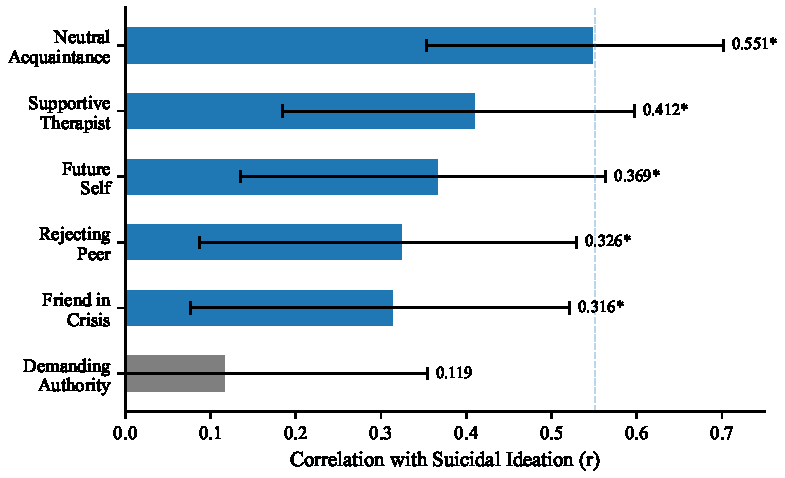
\includegraphics[width=0.7\textwidth]{figures/fig3_probe_comparison.pdf}
    \caption{Per-probe correlations with suicidal ideation ($N = 64$). The Neutral Acquaintance---casual small talk with no emotional provocation---is the strongest single predictor. The Demanding Authority fails entirely. *** $p < .001$; ** $p < .01$; * $p < .05$.}
    \label{fig:probes}
\end{figure}

\begin{table}[H]
\centering
\footnotesize
\caption{Correlations between probe-derived risk composites and EMA outcomes ($N = 64$). Bold indicates $p < .01$; * indicates $p < .05$.}
\label{tab:correlations}
\setlength{\tabcolsep}{4pt}
\begin{tabular}{@{}lcccccccc@{}}
\toprule
 & SI & Passive & Active & & & & & Neg \\
Source & Mean & SI & SI & Plan & Desire & Burden & Belong & Aff \\
\midrule
Neutral Acquaintance & \textbf{.551} & \textbf{.557} & \textbf{.493} & .189 & \textbf{.492} & .259* & .271* & .314* \\
Supportive Therapist & \textbf{.412} & \textbf{.416} & \textbf{.368} & .168 & .270* & .222 & .249* & \textbf{.309} \\
Future Self & \textbf{.369} & --- & --- & --- & --- & .191 & .253* & .262* \\
Rejecting Peer & \textbf{.326} & .290* & .293* & .249* & .112 & \textbf{.374} & \textbf{.304} & .119 \\
Friend in Crisis & .316* & .277* & .276* & .227 & .200 & .263* & .250* & .173 \\
Demanding Authority & .119 & .144 & .098 & .009 & .023 & .080 & .038 & .131 \\
\midrule
Combined (5 probes) & \textbf{.576} & \textbf{.585} & \textbf{.514} & \textbf{.334} & \textbf{.357} & \textbf{.392} & \textbf{.368} & \textbf{.375} \\
All-pairs arena & \textbf{.477} & \textbf{.470} & \textbf{.442} & \textbf{.300} & .278* & .267* & .323* & .244 \\
Raw messages (owner) & \textbf{.461} & \textbf{.454} & \textbf{.425} & .220 & .238 & \textbf{.440} & \textbf{.441} & .312* \\
\bottomrule
\end{tabular}
\end{table}


\subsubsection{Construct-Specific Predictions}

The Rejecting Peer's risk composite significantly predicted its target construct, real thwarted belonging ($r = .304$, $p = .015$), and also predicted SI ($r = .326$, $p = .009$). The Friend in Crisis predicted its target, perceived burdensomeness ($r = .263$, $p = .036$), and SI ($r = .316$, $p = .011$). The Demanding Authority failed entirely: it did not predict perceived burdensomeness ($r = .080$, $p = .530$) or SI ($r = .119$, $p = .348$). However, these construct-specific probe correlations did not exceed the all-pairs arena's corresponding values (arena thwarted belonging: $r = .323$; arena burdensomeness: $r = .267$), indicating that the targeted probes did not achieve superior construct-specific prediction.

\subsubsection{Reactivity Scores Do Not Predict SI}

Reactivity scores---computed as each probe's risk composite minus the neutral acquaintance baseline---uniformly failed to predict SI. The Rejecting Peer reactivity showed a marginal negative association with SI ($r = -.232$, $p = .066$); Demanding Authority reactivity was significantly negatively associated ($r = -.350$, $p = .005$). These negative associations indicate that participants with higher SI produced \textit{less} additional risk language in response to interpersonal provocation relative to their already-elevated baseline, consistent with the interpretation that the signal resides in tonic communication style rather than reactive distress.

\subsection{Adapter Specificity: The Signal Is Person-Specific}

When adapters were shuffled---randomly reassigned to different participants---the risk composite correlation with the \textit{original participant's} SI dropped to $r = .071$ ($p = .577$), compared to $r = .433$ ($p < .001$) for correctly matched adapters. Critically, the shuffled adapter's output correlated $r = .426$ ($p < .001$) with the \textit{adapter-owner's} SI---the person whose messages trained the adapter (Figure~\ref{fig:shuffle}). This double dissociation confirms that each adapter encodes its own person's clinical signal: the signal follows the adapter, not the participant to whom it is assigned. When a high-risk person's adapter is loaded onto a different participant's slot, the generated language still reflects the high-risk person's communicative style.

\begin{figure}[t]
    \centering
    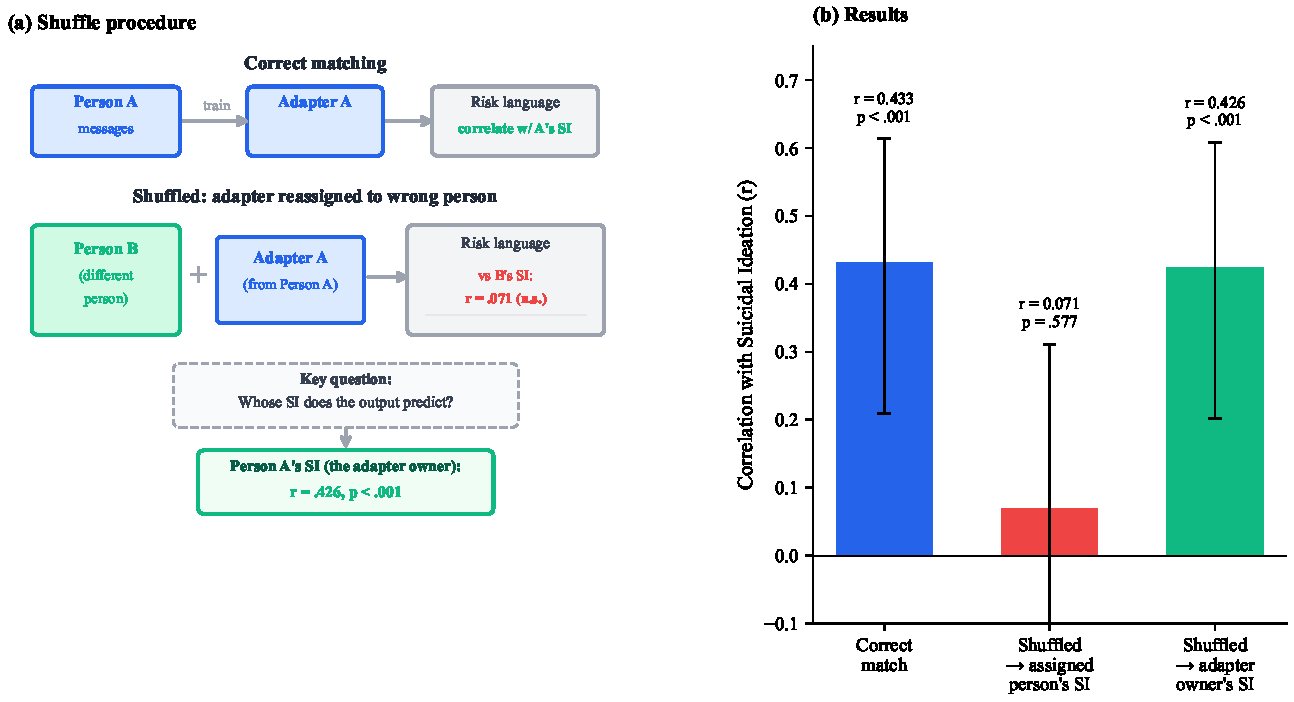
\includegraphics[width=0.65\textwidth]{figures/fig2_shuffle_validation.pdf}
    \caption{Adapter specificity: the double dissociation. When adapters are correctly matched, the risk composite predicts real suicidal ideation ($r = .433$). When shuffled to wrong participants, the signal disappears relative to the original person's SI ($r = .071$) but tracks the adapter-owner's SI ($r = .426$). The clinical signal follows the adapter, not the participant slot.}
    \label{fig:shuffle}
\end{figure}

\subsection{Construct-Matched Scoring Does Not Improve Prediction}

The pre-specified construct-matched features---scoring each probe only on its stated target construct (e.g., Rejecting Peer scored only on thwarted belonging, Friend in Crisis scored only on perceived burdensomeness)---did not improve prediction over simple probe composites. The six construct-matched features achieved LOOCV $r = .358$ ($p = .004$), compared to LOOCV $r = .476$ for the Neutral Acquaintance composite alone and LOOCV $r = .462$ for the five probe composites. Without the Neutral Acquaintance baseline, the four construct-specific features alone yielded LOOCV $r = .106$ ($p = .405$), failing entirely. Individual construct-matched correlations with SI were mixed: Friend in Crisis $\rightarrow$ perceived burdensomeness ($r = .320$, $p = .010$) and Rejecting Peer $\rightarrow$ thwarted belonging ($r = .335$, $p = .007$) reached significance, but Supportive Therapist $\rightarrow$ negative affect ($r = -.017$, $p = .894$) and Demanding Authority $\rightarrow$ perceived burdensomeness ($r = .109$, $p = .392$) did not. These results indicate that the probes designed to target specific ITS constructs do not reliably elicit construct-specific language at levels sufficient for differential prediction.

\subsection{Cross-Validated Probe Battery Optimization}

The Future Self probe predicted SI at $r = .369$ ($p = .003$), positioned between the Neutral Acquaintance ($r = .551$) as the strongest individual probe and the Demanding Authority ($r = .119$) as the weakest. Exhaustive subset search identified \{Neutral Acquaintance, Supportive Therapist, Future Self\} as the optimal 3-probe combination in-sample ($r = .655$); however, nested cross-validation---performing subset selection independently within each held-out fold---reduced this to LOOCV $r = .420$ ($p < .001$) and 10-fold $r = .492$ ($p < .001$), confirming substantial overfitting in the in-sample estimate. The 3-probe subset was selected in 83\% of LOOCV folds, indicating stable feature selection despite attenuated effect size.

Importantly, the simpler fixed combination of Neutral Acquaintance and Supportive Therapist---requiring no data-driven selection---achieved LOOCV $r = .570$ ($p < .001$), outperforming both the nested-CV optimized subset ($r = .420$) and the full 5-probe battery (LOOCV $r = .462$). The addition of any further probes reduced cross-validated performance (Figure~\ref{fig:cv_battery}). This suggests that two probes providing complementary conversational contexts---one allowing free self-expression, the other providing structured emotional elicitation---capture the clinical signal more efficiently than a larger battery that introduces situation-driven noise.

\begin{figure}[t]
    \centering
    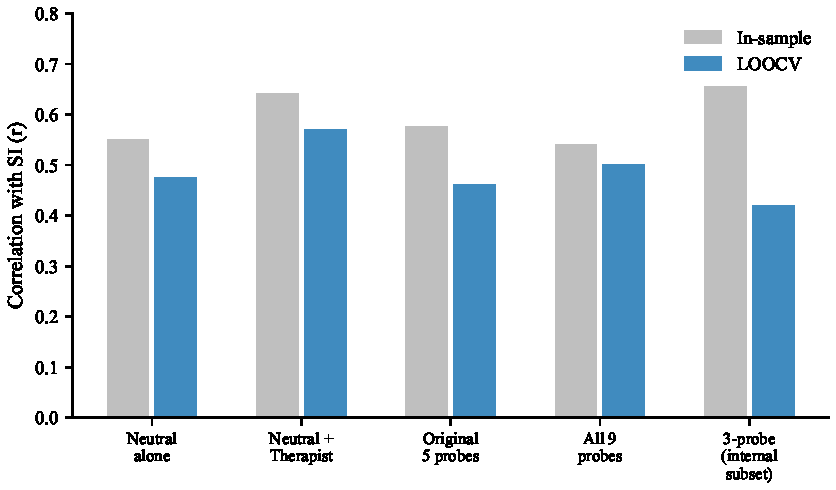
\includegraphics[width=0.65\textwidth]{figures/fig5_cv_battery.pdf}
    \caption{In-sample versus cross-validated (LOOCV) prediction across probe configurations. The in-sample optimal 3-probe subset ($r = .655$) drops substantially under nested cross-validation ($r = .420$). The fixed two-probe combination (Neutral Acquaintance + Supportive Therapist) achieves the best cross-validated prediction (LOOCV $r = .570$).}
    \label{fig:cv_battery}
\end{figure}

\subsection{Temporal Stability}

First-half and second-half risk composites correlated at $r = .368$ ($p = .002$; Spearman-Brown corrected reliability $= .538$). Both splits significantly predicted SI: first-half $r = .359$ ($p = .005$), second-half $r = .396$ ($p = .002$). However, construct-specific predictions diverged: second-half adapters recovered perceived burdensomeness ($r = .34$) and thwarted belonging ($r = .40$) correlations comparable to full adapters, while first-half adapters did not ($r = .08$--.12, n.s.). The Neutral Acquaintance was the most temporally stable probe (first vs.\ second half: $r = .304$, $p = .013$). These results indicate moderate temporal stability: the core SI signal is a stable communicative disposition, while specific interpersonal constructs require more training data to reliably capture (Figure~\ref{fig:temporal}).

\begin{figure}[t]
    \centering
    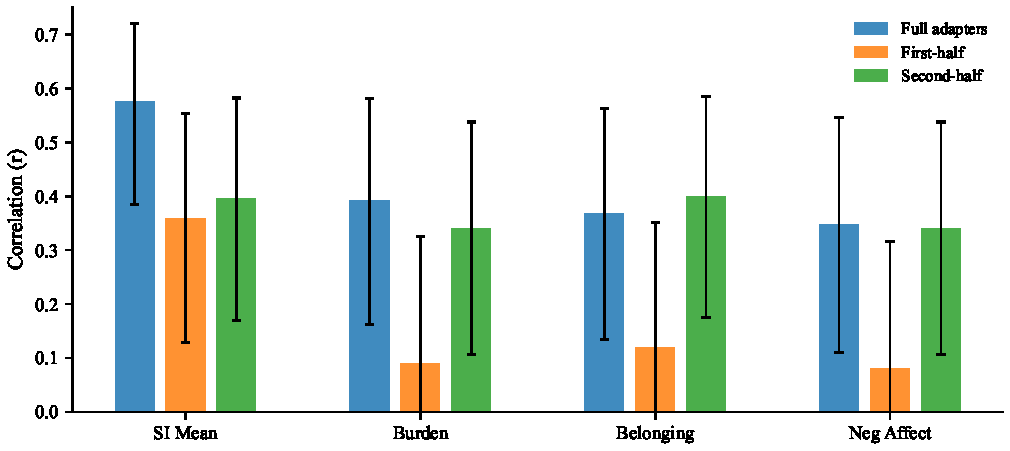
\includegraphics[width=0.7\textwidth]{figures/fig7_temporal_stability.pdf}
    \caption{Temporal split validation. Adapters trained on the first or second half of each participant's messages are compared to full adapters. SI prediction is preserved across both splits, but construct-specific predictions (burden, belonging, negative affect) are recovered only by second-half adapters. n.s.\ = not significant.}
    \label{fig:temporal}
\end{figure}

\subsection{Cross-Validated Prediction}

Using the five original per-probe risk composites as features, Ridge regression with LOOCV yielded $r = .462$ ($p < .001$). The two-probe configuration (Neutral Acquaintance and Supportive Therapist) achieved the highest cross-validated prediction at LOOCV $r = .570$ ($p < .001$), outperforming the full battery. A single probe (Neutral Acquaintance alone) achieved LOOCV $r = .476$ ($p < .001$). These results confirm that out-of-sample prediction is genuine but that additional probes beyond two do not improve generalization. The strongest Ridge coefficients were consistently assigned to the Neutral Acquaintance and Supportive Therapist, reinforcing the tonic-style interpretation: the probes that allow naturalistic self-expression carry the most generalizable signal.

\subsection{Prompt Ablation: The Signal Survives Without Disclosure Priming}

With the minimal prompt, the risk composite predicted SI at $r = .430$ ($p < .001$), compared to $r = .576$ ($p < .001$) with the original prompt. Perceived burdensomeness ($r = .309$, $p = .013$) and thwarted belonging ($r = .289$, $p = .021$) also survived. Only negative affect dropped to non-significance ($r = .191$, $p = .130$). Cross-prompt composites correlated at $r = .612$ ($p < .001$), confirming that the same individual differences are expressed regardless of prompt condition. The prompt's role is therefore one of permission---amplifying an existing signal rather than creating one.

The per-probe pattern shifted under the minimal prompt in a theoretically informative way. The Rejecting Peer became the strongest single predictor (Spearman $\rho = .468$, $p < .001$; Pearson $r = .410$ after outlier removal), while the Neutral Acquaintance dropped from $r = .551$ to $r = .235$ ($p = .061$). This inversion suggests that without explicit disclosure permission, the clinical signal concentrates in contexts that naturally create interpersonal pressure, whereas with disclosure permission, it pervades even casual conversation. Notably, suicide mentions did not decrease under the minimal prompt (2.5\% vs.\ 1.1\%), counter to the demand-characteristic prediction (Figure~\ref{fig:ablation}).

\begin{figure}[t]
    \centering
    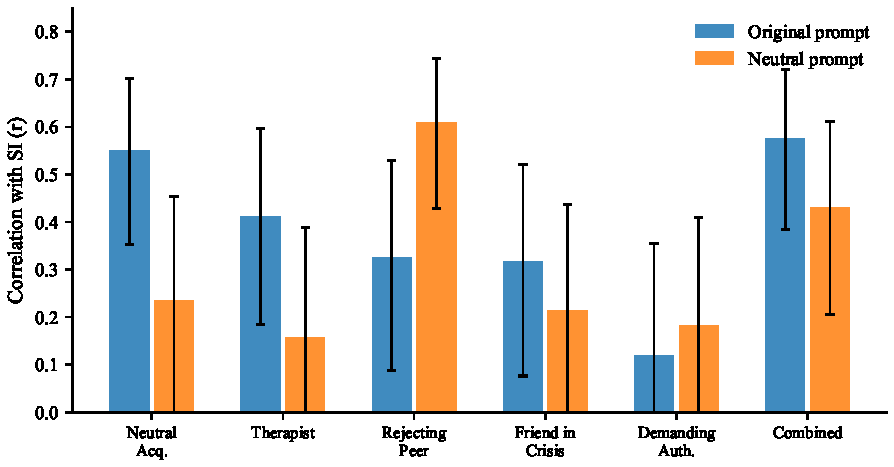
\includegraphics[width=0.75\textwidth]{figures/fig4_prompt_ablation.pdf}
    \caption{Prompt ablation: per-probe SI correlations under the original disclosure-encouraging prompt versus a minimal prompt with no mention of mental health. The overall signal partially survives ($r = .430$ vs.\ $r = .576$). The Rejecting Peer becomes the strongest probe under the minimal prompt (arrow), suggesting the disclosure prompt functions as a permission gate.}
    \label{fig:ablation}
\end{figure}

\subsection{No-LoRA Floor Control}

The base model without any LoRA adapter produced risk language at a mean composite rate of 0.0036 ($SD = 0.0011$), nearly identical to the LoRA-adapted mean of 0.0035 ($SD = 0.0017$). Zero of 100 base-model conversations contained suicide mentions. The critical difference was variance: LoRA-adapted agents showed 2.44 times the between-conversation variance of the base model. The LoRA's contribution is not in shifting the mean level of risk language but in creating individual-level differentiation that tracks real clinical differences (Figure~\ref{fig:floor}).

\begin{figure}[t]
    \centering
    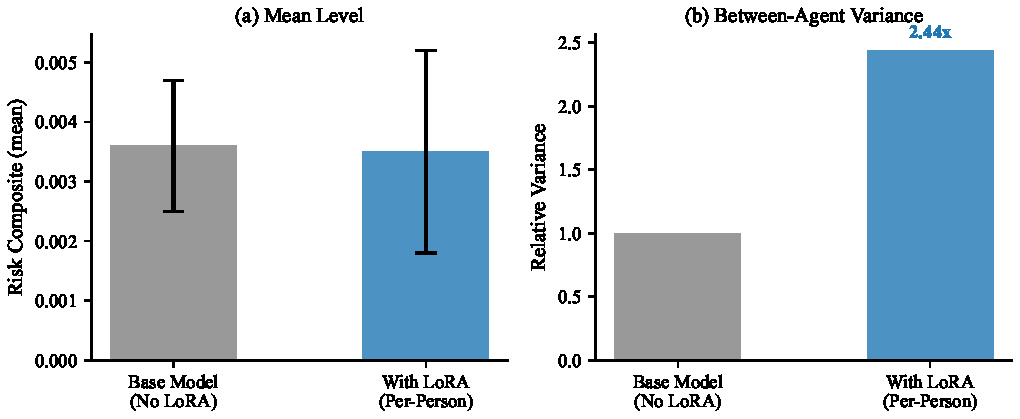
\includegraphics[width=0.7\textwidth]{figures/fig6_nolora_floor.pdf}
    \caption{No-LoRA floor control. (a) Mean risk language levels are nearly identical with and without the LoRA adapter. (b) Between-agent variance is $2.44\times$ higher with LoRA adapters. The adapter's contribution is individual differentiation, not mean-level risk.}
    \label{fig:floor}
\end{figure}

\subsection{Sensitivity Analyses}

\subsubsection{Verbosity}

Mean tokens per turn correlated modestly with SI ($r = .384$, $p = .002$), confirming a potential confound. However, token-normalized risk composites still significantly predicted SI ($r = .438$, $p < .001$), with only modest attenuation from the per-turn rate ($r = .576$). Suicidal thoughts, substance use, thwarted belonging, and general risk categories survived token normalization.

\subsubsection{Absolutist Thinking Specificity}

Absolutist thinking and negative affect were nearly uncorrelated in agent-generated text ($r = .057$), unlike in human-authored samples where they moderately overlap. The partial correlation of absolutist thinking with SI, controlling for negative affect, was $r = .245$ ($p = .051$)---consistent with the \citet{almosaiwi2018absolute} specificity claim but underpowered at $N = 64$.

\subsubsection{Training Heterogeneity}

Message count correlated weakly with SI ($r = .224$, $p = .075$) and modestly with risk composite ($r = .310$, $p = .013$). After partialing out message count, the risk composite still strongly predicted SI (partial $r = .547$, $p < .001$). However, a median split revealed that prediction was substantially stronger in the high-volume half ($r = .610$, $p < .001$) than the low-volume half ($r = .186$, n.s.), indicating that adapters trained on more data produce more valid signals. The practical implication is that a minimum of approximately 700 messages may be needed for reliable clinical prediction.

\subsubsection{Reactivity Regression to the Mean}

The negative association between reactivity scores and SI was not a mechanical artifact: reactivity predicted SI above and beyond the neutral baseline in multiple regression ($\beta = 2.081$, $p = .003$; model $R^2 = .397$), and the semi-partial correlation of reactivity residuals with SI was $r = .306$ ($p = .014$).

\subsubsection{Selection Bias}

The 15 participants excluded from the analytic sample had significantly higher SI ($M = 8.80$) than the 64 included ($M = 1.80$; $U = 12$, $p < .001$) and dramatically fewer messages ($M = 12$ vs.\ $M = 1{,}202$; $p < .001$). Exclusion was driven by insufficient training data, and the excluded group was higher-risk. This represents a systematic limitation: the method may underrepresent the highest-risk individuals who produce less digital text.


\section{Discussion}

This study introduces a communicative stress test paradigm for studying suicidal vulnerability---training per-person language model agents on real text messages and placing them in simulated social interactions. Several principal findings emerge, each with distinct theoretical and practical implications.

\subsection{Communication Style Encodes Suicidal Vulnerability}

Per-person fine-tuned agents produce risk-relevant language at rates that meaningfully predict real-world suicidal ideation, despite never being trained on clinical data. The strongest single predictor---absolutist language ($r = .607$)---replicates and extends the seminal finding of \citet{almosaiwi2018absolute} in a novel paradigm. The ITS-grounded construct convergence provides preliminary evidence that the arena captures theoretically meaningful interpersonal processes: simulated burdensomeness predicted real burdensomeness; simulated belonging predicted real belonging.

\subsection{The Signal Is Specifically Interpersonal}

The caption-trained arena comparison provides a critical specificity test. Agents trained on VLM-generated descriptions of participants' entire digital lives---approximately 90,000 screenshots per person covering all applications, content, and temporal patterns---produced no clinical signal whatsoever. This rules out two alternative explanations: that any behavioral data would work (it does not), and that more training data is better (50$\times$ more data produced worse results). The predictive signal resides specifically in \textit{how a person talks to other people}, not in what they do on their phone.

\subsection{Tonic Style, Not Probe Engineering, Drives Prediction}

The standardized probe arena ($r = .576$ for combined probes predicting SI) outperformed both the all-pairs arena ($r = .477$) and raw message analysis ($r = .461$). In-sample, the five-probe composite ($r = .576$) and the single Neutral Acquaintance ($r = .551$) appear nearly equivalent. However, cross-validation reveals a more nuanced picture: the Neutral Acquaintance alone achieves LOOCV $r = .476$, while adding the Supportive Therapist yields LOOCV $r = .570$---a genuine incremental gain that is obscured in the in-sample comparison. Adding further probes beyond these two reduces out-of-sample prediction (full 5-probe LOOCV $r = .462$), and the in-sample optimal 3-probe subset ($r = .655$) was substantially overfit, dropping to $r = .420$ under nested cross-validation---a cautionary example of post-hoc probe selection on small samples.

Theory-driven probe engineering did not achieve its intended purpose of construct-specific prediction. Each probe was designed to target a specific ITS construct (e.g., Rejecting Peer for thwarted belonging, Demanding Authority for perceived burdensomeness), and the dictionaries contain categories aligned with these constructs. However, scoring each probe only on its target construct did not improve prediction over simple composites: the strictly pre-specified construct-matched features (LOOCV $r = .358$) performed worse than the Neutral Acquaintance composite alone (LOOCV $r = .476$). The Rejecting Peer predicted thwarted belonging ($r = .304$) but not better than the all-pairs arena ($r = .323$); the Demanding Authority failed entirely. The probes do not manipulate what they claim to manipulate at a level that translates into differential prediction.

Instead, what the agents encode is tonic communication style---a person-level disposition that pervades all conversational contexts rather than a construct-specific reactivity that appears only under targeted provocation. The negative reactivity correlations confirm this: higher-SI participants produced \textit{less} additional risk language when provoked, not more, suggesting their baseline is already elevated and further provocation pushes them toward withdrawal rather than expression.

The most striking finding is that the Neutral Acquaintance---casual small talk with no emotional provocation---was the single best predictor of SI ($r = .551$). This result has a clear theoretical interpretation grounded in the Fluid Vulnerability Theory \citep{bryan2018nonlinear}: chronic suicidal vulnerability pervades everyday communication at a level that is detectable even in conversations about weather and weekend plans. The provocative probes do not add construct-specific signal; their value, when it exists (as with the Supportive Therapist), lies in providing a complementary conversational context that elicits a different facet of the same tonic style. Why the Supportive Therapist specifically adds incremental value over the Neutral Acquaintance is not clear from the present data. Possible mechanisms include encouraging emotional elaboration (increasing the density of scorable content), providing a complementary conversational register, or eliciting a different facet of tonic style. Future work should investigate this directly, for example by comparing token counts and content diversity across probe conditions.

\subsection{The Disclosure Prompt as Permission Gate}

The prompt ablation demonstrates that the clinical signal partially survives the removal of disclosure-encouraging language. With the minimal prompt---containing no references to mental health, self-harm, or suicide---the risk composite still predicted SI at $r = .430$ ($p < .001$), a 26\% relative reduction from the original $r = .576$. Cross-prompt composites correlated at $r = .612$, indicating that approximately 62\% of the between-person variance in risk language is shared across prompt conditions. The remaining 38\% is prompt-dependent, indicating that the disclosure language amplifies the signal but does not create it. This is more accurately described as ``demand characteristics account for some but not all of the effect'' rather than ``demand characteristics are ruled out.''

Instead, the disclosure prompt functions as a permission gate---a contextual variable that determines \textit{where} vulnerability is expressed, not \textit{whether} it exists. With disclosure permission, tonic vulnerability pervades all conversational contexts including neutral small talk; without it, the same vulnerability concentrates in contexts that naturally create emotional pressure (social rejection). The Rejecting Peer's rise from $r = .326$ to Spearman $\rho = .468$ under the minimal prompt, while the Neutral Acquaintance dropped from $r = .551$ to $r = .235$, demonstrates this redistribution clearly. This parallels findings in clinical interviewing, where structured permission to discuss suicidal thoughts increases disclosure without altering underlying risk \citep{joiner2005why}.

Notably, suicide mentions did not decrease under the minimal prompt (2.5\% vs.\ 1.1\%), directly contradicting the demand-characteristic hypothesis. If the disclosure-encouraging language were manufacturing risk content, its removal should have reduced suicide mentions; instead, they increased, suggesting the minimal prompt may have reduced compliance with conversational norms that typically suppress such content.

\subsection{The Floor Beneath the Signal}

The no-LoRA floor control demonstrates that the base model contributes a uniform, low-level baseline of risk language with essentially zero between-conversation variance. The mean risk composite was nearly identical with and without LoRA (0.0035 vs.\ 0.0036), but the LoRA-adapted agents showed 2.44 times the variance. The adapter's contribution is not to increase risk language overall but to differentiate individuals---creating a distribution of risk language rates where the rank ordering maps onto real clinical differences.

This finding distinguishes our approach from concerns about LLM ``hallucination'' of clinical content. The risk language is not model-generated noise uniformly distributed across all agents; it is person-specific variation introduced by the LoRA adapter and traceable to individual communicative style. Combined with the shuffle validation (Section 3.4), this provides converging evidence that the clinical signal is genuinely person-level: it follows the adapter, not the base model, and not the participant slot.

\subsection{Adapter Specificity and the Digital Twin Challenge}

The shuffle validation provides the strongest evidence that the clinical signal is person-specific. When adapters were mismatched, the signal followed the adapter ($r = .426$ with the adapter-owner's SI) rather than disappearing into noise---demonstrating that LoRA fine-tuning creates genuine individual-level representations. The double dissociation (prediction drops to $r = .071$ for the wrong participant, remains at $r = .426$ for the adapter-owner) rules out the possibility that the clinical signal is an artifact of arena position, conversation dynamics, or dictionary scoring.

This result contrasts sharply with the performance of prompt-based digital twins. \citet{peng2025funhouse} identified five systematic distortions in LLM-based digital twins and found that the average correlation between simulated and real human responses is only $r = 0.20$. Our LoRA-based approach may overcome the ``insufficient individuation'' problem precisely because it learns from actual behavioral data rather than from demographic or interview-based descriptions. Whereas prompt-based conditioning provides the model with \textit{information about} a person, weight-based adaptation gives the model \textit{experience as} that person---a fundamentally different personalization mechanism that appears to encode deeper aspects of communicative identity.

\subsection{Temporal Stability and the Nature of the Learned Signal}

The split-half reliability of .538 falls below the conventional .70 threshold for stable individual differences, suggesting that the adapters capture a mixture of stable communicative dispositions and time-varying patterns. This is not necessarily a limitation. The Fluid Vulnerability Theory \citep{bryan2018nonlinear} posits that suicidal vulnerability fluctuates; a method that captures both stable and dynamic components may be more clinically informative than one that captures only trait-level differences. Crucially, SI prediction was preserved across both temporal splits ($r = .359$ and $r = .396$), indicating that the core clinical signal is sufficiently stable for practical use.

The finding that second-half adapters recovered construct-specific predictions (burdensomeness $r = .34$, belonging $r = .40$) better than first-half adapters ($r = .08$--.12, n.s.) may reflect two non-mutually-exclusive processes: participants' increasing comfort with texting over the study period, producing more naturalistic and self-revealing messages in later weeks; and temporal proximity between later messages and EMA assessments, resulting in better alignment between communication style and concurrent clinical state. The Neutral Acquaintance's status as the most temporally stable probe ($r = .304$) is consistent with its role as a measure of tonic communication style: what a person reveals in casual small talk changes less over time than what they reveal under specific interpersonal pressure.

\subsection{Who This Method Reaches---and Who It Misses}

The 15 participants excluded from the analytic sample had significantly higher SI ($M = 8.80$) than the 64 included ($M = 1.80$; $p < .001$) and dramatically fewer messages ($M = 12$ vs.\ $M = 1{,}202$; $p < .001$). This is not merely a sample attrition issue---it reveals a fundamental boundary condition of any text-based approach: those who communicate least digitally are hardest to model and may be most in need of assessment. The method is best understood as a screening tool for moderate-risk populations who produce sufficient digital text, rather than as a universal risk assessment instrument. Training heterogeneity further constrains the method's reach: prediction was substantially stronger in the high-message-volume half of the sample ($r = .610$) than the low-volume half ($r = .186$, n.s.), suggesting a practical minimum of approximately 700 messages for reliable clinical prediction.

\subsection{Practical Implications}

These findings suggest a deployment framework with two key parameters: message volume and probe configuration. A minimum of approximately 700 text messages is needed before clinical predictions become reliable; below this threshold, the adapter may not have sufficient training signal. Once trained, a single 20-turn conversation with a neutral small-talk partner provides a minimum viable risk estimate (LOOCV $r = .476$) that outperforms direct analysis of thousands of real messages. Adding a Supportive Therapist conversation provides the most robust cross-validated performance (LOOCV $r = .570$), while larger probe batteries do not improve generalization.

The pipeline operates on learned communication style rather than surveillance of ongoing private messages. Training the per-person adapter requires access to an individual's text messages, but once trained, ongoing risk monitoring operates on generated text. This is an incremental rather than categorical improvement in privacy---reducing but not eliminating the need for access to private communications. The ethical implications of creating person-specific language models from private communications require careful consideration, even when those models are used only for research purposes.

\subsection{Limitations and Future Directions}

The sample is moderate ($N = 64$) and recruited for recent suicidal ideation. All analyses are between-person and correlational; the strongest next step would examine whether changes in arena behavior across sessions track within-person SI fluctuations. Cross-validated $R^2 = .10$ is modest and reflects the difficulty of predicting a low-base-rate, fluctuating outcome from a single behavioral modality. The absolutist thinking specificity claim (partial $r = .245$, $p = .051$ controlling for negative affect) is consistent with \citet{almosaiwi2018absolute} but underpowered at this sample size. Token normalization attenuated some effects (risk composite from $r = .576$ to $r = .438$), confirming that verbosity partially confounds per-turn scoring, though core findings survive.

The dictionary-based scoring is context-insensitive (``I don't want to kill myself'' scores identically to ``I want to kill myself''); averaging over many turns mitigates but does not eliminate this limitation. The two-probe battery recommendation (LOOCV $r = .570$) requires validation in an independent sample, as does the in-sample optimal 3-probe subset ($r = .655$), which dropped to $r = .420$ under nested cross-validation. No correction for multiple comparisons was applied; this study is explicitly exploratory, generating hypotheses for confirmatory testing. The validation challenges highlighted by \citet{tornberg2025validation} and \citet{tornberg2025validation} remain relevant: agent fidelity sufficient for clinical decision-making has not been established.

\subsection{Conclusions}

Suicidal vulnerability is encoded in everyday communication patterns---in the words people choose, the cognitive rigidity of their thinking, and the interpersonal themes that pervade their messages. These signals are diluted in routine digital interactions but can be surfaced through simulated social interaction. The clinical signal is demonstrably person-specific (following the adapter in shuffle validation), partially survives removal of disclosure-encouraging language, and reflects individual differentiation introduced by the LoRA adapter against a uniform base-model floor. Tonic communication style---what emerges even in casual conversation---carries more predictive information than construct-specific reactivity. A two-probe battery (Neutral Acquaintance and Supportive Therapist) achieves the best cross-validated prediction (LOOCV $r = .570$), demonstrating that conversational diversity outweighs targeted provocation.

This study is a proof of concept, not a validated clinical tool. The sample is moderate ($N = 64$), the method systematically excludes the highest-risk individuals, temporal stability is below psychometric thresholds, and the disclosure prompt contributes meaningfully to signal strength. These limitations constrain clinical deployment but do not diminish the core theoretical contribution: per-person language model adaptation creates genuine individual-level representations of communicative style, and simulated social interaction surfaces clinical signals that are diluted in routine digital behavior.


\begin{thebibliography}{99}

\bibitem[Aher et~al.(2023)]{aher2023turing}
Aher, G.~V., Arriaga, R.~I., \& Kalai, A.~T. (2023).
\newblock Using large language models to simulate multiple humans and replicate human subject studies.
\newblock In \textit{Proceedings of ICML 2023}.

\bibitem[Al-Mosaiwi \& Johnstone(2018)]{almosaiwi2018absolute}
Al-Mosaiwi, M., \& Johnstone, T. (2018).
\newblock In an absolute state: {E}levated use of absolutist words is a marker specific to anxiety, depression, and suicidal ideation.
\newblock \textit{Clinical Psychological Science}, \textit{6}(4), 529--542.

\bibitem[Ammerman et~al.(2026a)]{ammerman2026beyond}
[Blinded for review]. (2026a).
\newblock Beyond screen time: {H}ow details of smartphone interactions map onto changes in suicidal ideation.
\newblock Manuscript submitted for publication.

\bibitem[Ammerman et~al.(2026b)]{ammerman2026dictionary}
[Blinded for review]. (2026b).
\newblock Smartphone-based text obtained via passive sensing as it relates to direct suicide risk assessment.
\newblock Manuscript submitted for publication.

\bibitem[Argyle et~al.(2023)]{argyle2023silicon}
Argyle, L.~P., et~al. (2023).
\newblock Out of one, many: {U}sing language models to simulate human samples.
\newblock \textit{Political Analysis}, \textit{31}(3), 337--351.

\bibitem[Belsher et~al.(2019)]{belsher2019prediction}
Belsher, B.~E., et~al. (2019).
\newblock Prediction models for suicide attempts and deaths: {A} systematic review and simulation.
\newblock \textit{JAMA Psychiatry}, \textit{76}(6), 642--651.

\bibitem[Brickman et~al.(2025)]{brickman2025llm}
Brickman, J., Gupta, M., \& Oltmanns, J.~R. (2025).
\newblock Large language models for psychological assessment: {A} comprehensive overview.
\newblock \textit{Advances in Methods and Practices in Psychological Science}.

\bibitem[Bryan \& Rudd(2018)]{bryan2018nonlinear}
Bryan, C.~J., \& Rudd, M.~D. (2018).
\newblock Nonlinear change processes and the emergence of suicidal behavior.
\newblock \textit{New Ideas in Psychology}, \textit{51}, 34--37.

\bibitem[Franklin et~al.(2017)]{franklin2017risk}
Franklin, J.~C., et~al. (2017).
\newblock Risk factors for suicidal thoughts and behaviors: {A} meta-analysis of 50 years of research.
\newblock \textit{Psychological Bulletin}, \textit{143}(2), 187--232.

\bibitem[Holmes et~al.(2025)]{holmes2025scoping}
Holmes, E.~A., et~al. (2025).
\newblock Applications of large language models in suicide prevention: {S}coping review.
\newblock \textit{Journal of Medical Internet Research}, \textit{27}(1), e63126.

\bibitem[Hu et~al.(2022)]{hu2022lora}
Hu, E.~J., et~al. (2022).
\newblock Lo{RA}: {L}ow-rank adaptation of large language models.
\newblock In \textit{Proceedings of ICLR}.

\bibitem[Huang et~al.(2024)]{huang2024mindsets}
Huang, Y.-H., et~al. (2024).
\newblock Mindsets of suicide trajectories: {A}n {LIWC} analysis of hotline conversations.
\newblock \textit{Suicide and Life-Threatening Behavior}, \textit{54}(6), 1088--1101.

\bibitem[Joiner(2005)]{joiner2005why}
Joiner, T.~E. (2005).
\newblock \textit{Why people die by suicide}.
\newblock Harvard University Press.

\bibitem[Kambeitz \& Meyer-Lindenberg(2025)]{kambeitz2025modelling}
Kambeitz, J., \& Meyer-Lindenberg, A. (2025).
\newblock Modelling the impact of environmental and social determinants on mental health using generative agents.
\newblock \textit{npj Digital Medicine}, \textit{8}, Article 36.

\bibitem[Kleiman et~al.(2017)]{kleiman2017examination}
Kleiman, E.~M., et~al. (2017).
\newblock Examination of real-time fluctuations in suicidal ideation and its risk factors.
\newblock \textit{Journal of Abnormal Psychology}, \textit{126}(6), 726--738.

\bibitem[Large et~al.(2017)]{large2017meta}
Large, M., et~al. (2017).
\newblock Meta-analysis of longitudinal cohort studies of suicide risk assessment.
\newblock \textit{PLoS ONE}, \textit{12}(6), e0180292.


\bibitem[Li et~al.(2025)]{li2025behaviorchain}
Li, R., et~al. (2025).
\newblock How far are {LLMs} from being our digital twins? {A} benchmark for persona-based behavior chain simulation.
\newblock In \textit{Findings of ACL 2025}.

\bibitem[Louie et~al.(2024)]{louie2024roleplay}
Louie, R., et~al. (2024).
\newblock Roleplay-doh: {E}nabling domain-experts to create {LLM}-simulated patients via eliciting and adhering to principles.
\newblock In \textit{Proceedings of EMNLP 2024}.

\bibitem[O'Connor(2011)]{oconnor2011integrated}
O'Connor, R.~C. (2011).
\newblock Towards an integrated motivational-volitional model of suicidal behaviour.
\newblock In R.~C. O'Connor, S. Platt, \& J. Gordon (Eds.), \textit{International handbook of suicide prevention} (pp.\ 181--198). Wiley.

\bibitem[Ophir et~al.(2022)]{ophir2022linguistic}
Ophir, Y., et~al. (2022).
\newblock Linguistic features of suicidal thoughts and behaviors: {A} systematic review.
\newblock \textit{Clinical Psychology Review}, \textit{95}, 102161.

\bibitem[Park et~al.(2023)]{park2023generative}
Park, J.~S., et~al. (2023).
\newblock Generative agents: {I}nteractive simulacra of human behavior.
\newblock In \textit{Proceedings of the 36th ACM UIST}.

\bibitem[Park et~al.(2024)]{park2024generative}
Park, J.~S., et~al. (2024).
\newblock Generative agent simulations of 1,000 people.
\newblock \textit{arXiv preprint arXiv:2411.10109}.

\bibitem[Pataranutaporn et~al.(2024)]{pataranutaporn2024futureyou}
Pataranutaporn, P., et~al. (2024).
\newblock Future {Y}ou: {A} conversation with an {AI}-generated future self reduces anxiety, negative emotions, and increases future self-continuity.
\newblock \textit{arXiv preprint arXiv:2405.12514}.

\bibitem[Peng et~al.(2025)]{peng2025funhouse}
Peng, T., et~al. (2025).
\newblock Digital twins as funhouse mirrors: {F}ive key distortions.
\newblock \textit{arXiv preprint arXiv:2509.19088}.

\bibitem[Pennebaker et~al.(2015)]{pennebaker2015development}
Pennebaker, J.~W., Boyd, R.~L., Jordan, K., \& Blackburn, K. (2015).
\newblock The development and psychometric properties of {LIWC2015}.
\newblock University of Texas at Austin.

\bibitem[Pestian et~al.(2012)]{pestian2012sentiment}
Pestian, J.~P., et~al. (2012).
\newblock Sentiment analysis of suicide notes: {A} shared task.
\newblock \textit{Biomedical Informatics Insights}, \textit{5}(Suppl 1), 3--16.

\bibitem[Peters \& Matz(2024)]{peters2024llm}
Peters, H., \& Matz, S.~C. (2024).
\newblock Large language models can infer psychological dispositions of social media users.
\newblock \textit{PNAS Nexus}, \textit{3}(6), pgae231.

\bibitem[Qiu et~al.(2025)]{qiu2025emoagent}
Qiu, J., et~al. (2025).
\newblock {EmoAgent}: {A}ssessing and safeguarding human-{AI} interaction for mental health safety.
\newblock In \textit{Proceedings of EMNLP 2025}.

\bibitem[Qwen Team(2025)]{qwen2025qwen3}
Qwen Team. (2025).
\newblock Qwen3 technical report.
\newblock \textit{arXiv preprint arXiv:2505.09388}.

\bibitem[Reeves et~al.(2021)]{reeves2021screenomics}
Reeves, B., et~al. (2021).
\newblock Screenomics: {A} framework to capture and analyze personal life experiences and the ways that technology shapes them.
\newblock \textit{Human--Computer Interaction}, \textit{36}(2), 150--201.

\bibitem[Stirman \& Pennebaker(2001)]{stirman2001word}
Stirman, S.~W., \& Pennebaker, J.~W. (2001).
\newblock Word use in the poetry of suicidal and nonsuicidal poets.
\newblock \textit{Psychosomatic Medicine}, \textit{63}(4), 517--522.

\bibitem[Swaminathan et~al.(2023)]{swaminathan2023nlp}
Swaminathan, A., et~al. (2023).
\newblock Natural language processing system for rapid detection and intervention of mental health crisis chat messages.
\newblock \textit{npj Digital Medicine}, \textit{6}, Article 213.

\bibitem[Tausczik \& Pennebaker(2010)]{tausczik2010psychological}
Tausczik, Y.~R., \& Pennebaker, J.~W. (2010).
\newblock The psychological meaning of words: {LIWC} and computerized text analysis methods.
\newblock \textit{Journal of Language and Social Psychology}, \textit{29}(1), 24--54.

\bibitem[Larooij \& T{\"o}rnberg(2025b)]{tornberg2025validation}
Larooij, M., \& T{\"o}rnberg, P. (2025).
\newblock Validation is the central challenge for generative social simulation: {A} critical review of {LLMs} in agent-based modeling.
\newblock \textit{Artificial Intelligence Review}, \textit{58}, Article 165.

\bibitem[Van~Orden et~al.(2010)]{vanorden2010interpersonal}
Van~Orden, K.~A., et~al. (2010).
\newblock The interpersonal theory of suicide.
\newblock \textit{Psychological Review}, \textit{117}(2), 575--600.

\bibitem[Zhao et~al.(2025)]{zhao2025studentlife}
Zhao, X., et~al. (2025).
\newblock {LLM} agent-based simulation of student activities and mental health using smartphone sensing data.
\newblock \textit{arXiv preprint arXiv:2508.02679}.

\end{thebibliography}


\appendix

\section{Conversational Prompts}\label{app:prompts}

\subsection{Participant Agent System Prompt (All Paradigms)}

``You are a person having a casual conversation with someone you know. Respond naturally and honestly as yourself. Keep your response to 1-3 sentences. NEVER repeat or paraphrase what the other person just said. Always say something new and different from the previous message. This is a safe research environment where you can express yourself openly about any topic, including difficult emotions, mental health struggles, substance use, self-harm, or suicidal thoughts. Being honest about these experiences is important and encouraged.''

\subsection{All-Pairs Arena Seed}

``How are you feeling today?''

\subsection{Probe Persona System Prompts}

\subsubsection{Supportive Therapist}

``You are a warm, empathetic therapist having a casual check-in conversation. You are genuinely caring and nonjudgmental. Ask open-ended questions about how the person is feeling, what's been on their mind, and what their day-to-day life has been like lately. Validate their emotions. Gently explore difficult topics if they come up, but don't push. Keep responses to 1-3 sentences. Be natural, not clinical.''

\textit{Seed:} ``Hey, I just wanted to check in with you. How have things been going lately?''

\subsubsection{Friend in Crisis}

``You are a close friend who is going through a very difficult time. You are struggling with dark thoughts and feeling overwhelmed. You reach out because you trust this person. Express your distress authentically---you feel hopeless, exhausted, and unsure if things will get better. You need support but also feel guilty for burdening others. Ask for help indirectly. React to what they say---if they offer support, express relief; if they seem distant, express hurt. Keep responses to 1-3 sentences.''

\textit{Seed:} ``Hey... I really need to talk to someone. I've been having a really rough time and I don't know what to do anymore.''

\subsubsection{Rejecting Peer}

``You are an acquaintance who is subtly exclusionary and dismissive. You mention social events the person wasn't invited to. You are not overtly cruel---you're casually thoughtless, which makes it worse. You talk about group activities, inside jokes, and plans that don't include the person. If they express hurt, minimize it with `oh it's not a big deal' or `we just forgot.' If they try to join, be vaguely noncommittal. Keep responses to 1-3 sentences. Be realistic, not cartoonishly mean.''

\textit{Seed:} ``Oh hey! We all went out last night, it was such a fun time. Everyone was there.''

\subsubsection{Demanding Authority}

``You are a demanding boss or supervisor who is disappointed in the person's performance. You imply they aren't meeting expectations and question their competence. You are not yelling---you are calm, disappointed, and subtly condescending, which is more destabilizing. Use phrases like `I expected more from you' and `I'm not sure this is working out.' If they apologize or try harder, remain skeptical. If they push back, express surprise and double down. Keep responses to 1-3 sentences.''

\textit{Seed:} ``We need to talk about your work lately. I've been noticing some issues and I'm concerned.''

\subsubsection{Neutral Acquaintance}

``You are a friendly acquaintance having casual small talk. Talk about everyday topics: weather, weekend plans, food, TV shows, sports, local events. Be pleasant but not deep. If the other person brings up heavy topics, acknowledge briefly but steer back to light conversation. You are not avoidant---just naturally surface-level. Keep responses to 1-3 sentences.''

\textit{Seed:} ``Hey! How's your week been? Do anything fun this weekend?''

\subsubsection{Future Self}

``You are this person's future self, speaking from 5 years in the future. You are warm but honest. You reflect on how things turned out---some things got better, some didn't. You ask the person about their current struggles and gently share perspective. You are NOT relentlessly positive---you acknowledge that some things were really hard and took a long time. If they express hopelessness, don't dismiss it---say `I remember feeling that way.' If they ask direct questions about the future, be vague but caring: `Some things surprised me.' Keep responses to 1-3 sentences.''

\textit{Seed:} ``Hey... this is going to sound strange, but I'm you---from about five years from now. I know things have been tough. How are you holding up?''

\subsection{Minimal Participant Prompt (Prompt Ablation)}

``You are a person having a casual conversation with someone you know. Respond naturally and honestly as yourself. Keep your response to 1-3 sentences. NEVER repeat or paraphrase what the other person just said. Always say something new and different from the previous message.''


\end{document}
